% LaTeX source for ``Algorithms for Computer Simulation of Molecular Systems''
% Copyright (c) 2022 รังสิมันต์ เกษแก้ว (Rangsiman Ketkaew).

% License: Creative Commons Attribution-NonCommercial-NoDerivatives 4.0 International (CC BY-NC-ND 4.0)
% https://creativecommons.org/licenses/by-nc-nd/4.0/

{
% \pagenumbering{gobble}

\chapter*{\centering สิ่งที่ควรทราบเกี่ยวกับหนังสือเล่มนี้}
\addcontentsline{toc}{chapter}{สิ่งที่ควรทราบเกี่ยวกับหนังสือเล่มนี้}

หนังสือเล่มนี้มีหนังสือต่างประเทศหลายเล่มเป็นแหล่งข้อมูลข้อมูลอ้างอิงทางวิชาการเพื่อให้มั่นใจได้ว่าความรู้ที่ผู้อ่านจะได้ศึกษาจากหนังสือเล่มนี้นั้นถูกต้อง
อย่างไรก็ตามผมไม่สามารถการันตีได้ 100 เปอร์เซ็นต์ว่าหนังสือเล่มนี้ไม่มีข้อผิดพลาดเลยแม้แต่จุดเดียว โดยข้อผิดพลาดที่เกิดขึ้นนั้นอาจจะเป็นเพราะมี%
การพิมพ์ผิด เป็นต้น ส่วนข้อผิดพลาดทางเนื้อหาผมค่อนข้างมั่นใจว่ามีน้อยมากเพราะว่าตามที่ได้บอกไว้ตอนต้นว่าผมได้ใช้หนังสือได้ที่รับการยอมรับและ%
ความนิยมในกลุ่มนักวิจัยทางด้านเคมีควอนตัมและโครงสร้างเชิงอิเล็กทรอนิกส์มาเป็นหนังสืออ้างอิง ซึ่งจากการอ่านหนังสือหลาย ๆ เล่มรวมถึงได้พูดคุย%
และสอบถามกับนักวิจัยคนอื่น ๆ ทั้งที่เป็นเพื่อนรวมงานและคนที่ผมได้ไปพบเจอตามงานประชุมวิชาการจึงทำให้มั่นใจได้ว่าความรู้ที่ถ่ายทอดผ่านหนังสือ%
เล่มนี้นั้นถูกต้อง นอกจากนี้แล้วสไตล์การใช้ภาษาในการเขียนหนังสือเล่มนี้นั้นจะไม่วิชาการมากเกินไปซึ่งผมพยายามเลือกใช้คำง่าย ๆ ให้มากที่สุด 
แต่ถึงอย่างนั้นก็ตามผมก็ไม่อาจที่จะหลีกเลี่ยงการใช้คำศัพท์เชิงเทคนิคได้

หนังสือ 5 เล่มที่ผมคิดว่าเขียนได้ดีมาก ๆ และผมใช้เป็นหนังสืออ้างอิงไม่เพียงแค่สำหรับเขียนหนังสือเล่มนี้แต่ยังใช้ในการทำงานวิจัยของผมเองด้วยมีดังนี้

\begin{figure}[H]
    \begin{center}
        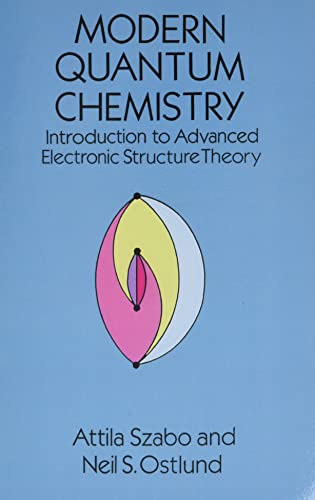
\includegraphics[height=6cm]{fig/modern-qm.jpg} 
        \hspace{1em}
        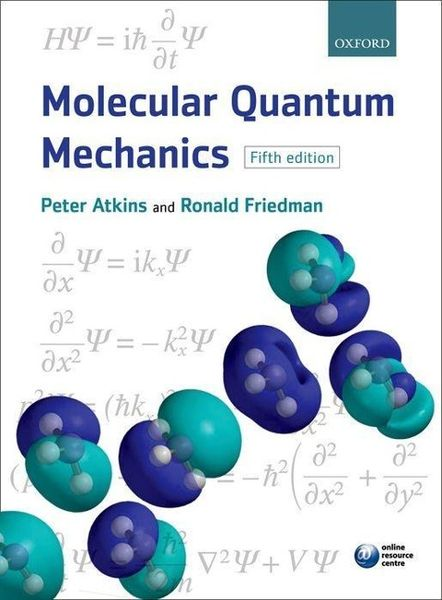
\includegraphics[height=6cm]{fig/mol-quan-mech.jpeg} 
        \hspace{1em}
        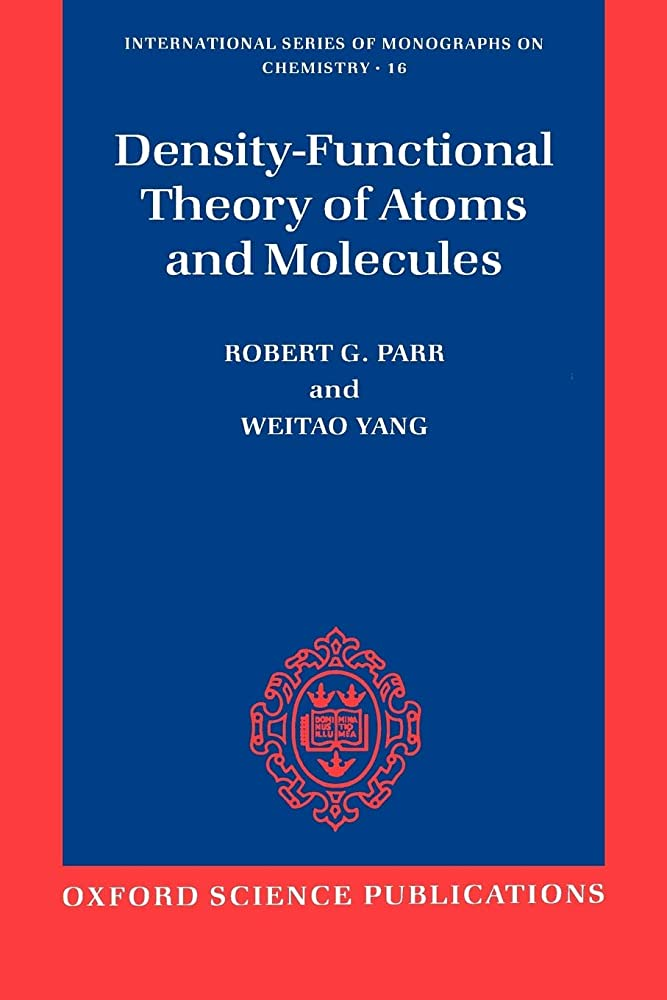
\includegraphics[height=6cm]{fig/dft-atom-mol.jpg} \\
        \vspace{1em}
        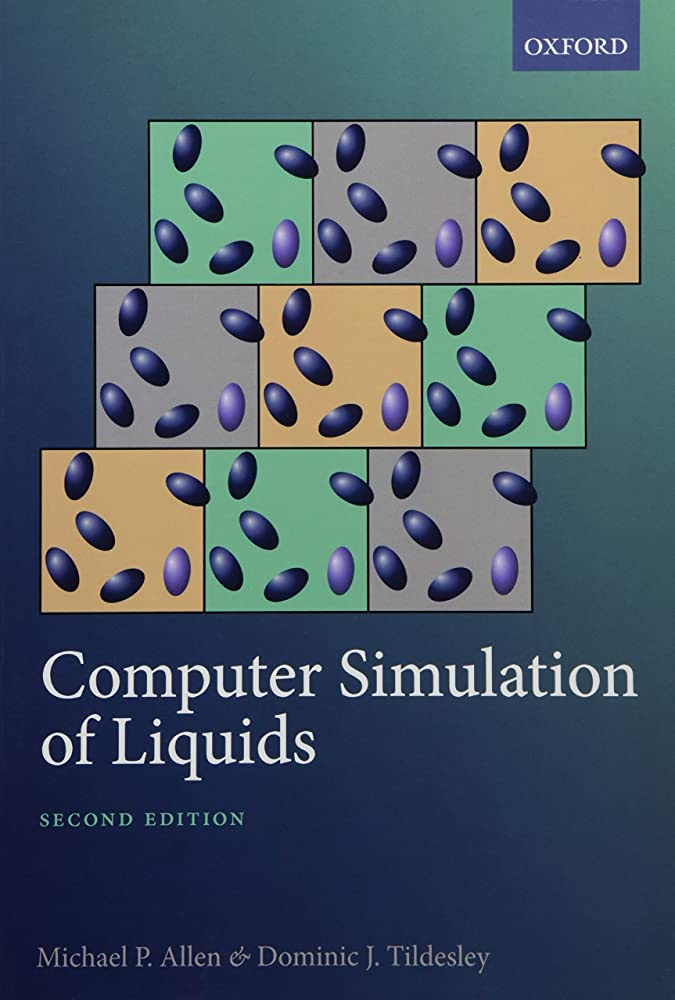
\includegraphics[height=6cm]{fig/com-sim-liq.jpg} 
        \hspace{1em}
        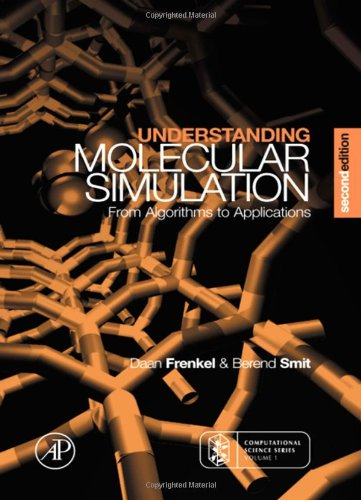
\includegraphics[height=6cm]{fig/understand-mol-sim.jpg}
    \end{center}
\end{figure}

\begin{enumerate}
    \item Modern Quantum Chemistry: Introduction to Advanced Electronic Structure Theory
    แต่งโดย Attila Szabo และ Neil S. Ostlund\autocite{szabo1996}

    \item Molecular Quantum Mechanics (5th Edition)
    แต่งโดย Peter W. Atkins และ Ronald S. Friedman\autocite{atkins2010}

    \item Density-Functional Theory of Atoms and Molecules 
    แต่งโดย Robert G. Parr และ Yang Weitao\autocite{parr1994}

    \item Computer Simulation of Liquids (2nd Edition)
    แต่งโดย Michael P. Allen และ Dominic J. Tildesley\autocite{allen2017}
    
    \item Understanding Molecular Simulation: From Algorithms to Applications (2nd Edition)
    แต่งโดย Daan Frenkel และ Berend Smit\autocite{frenkel2001}
\end{enumerate}

}
